\section{Struttura precedente}

La struttura sulla quale mi sono basato per il mio progetto si trova sul lago di Endine  precisamente nel comune di Spinone in via Nazionale 56. 

\begin{figure}[H]
	\centering
	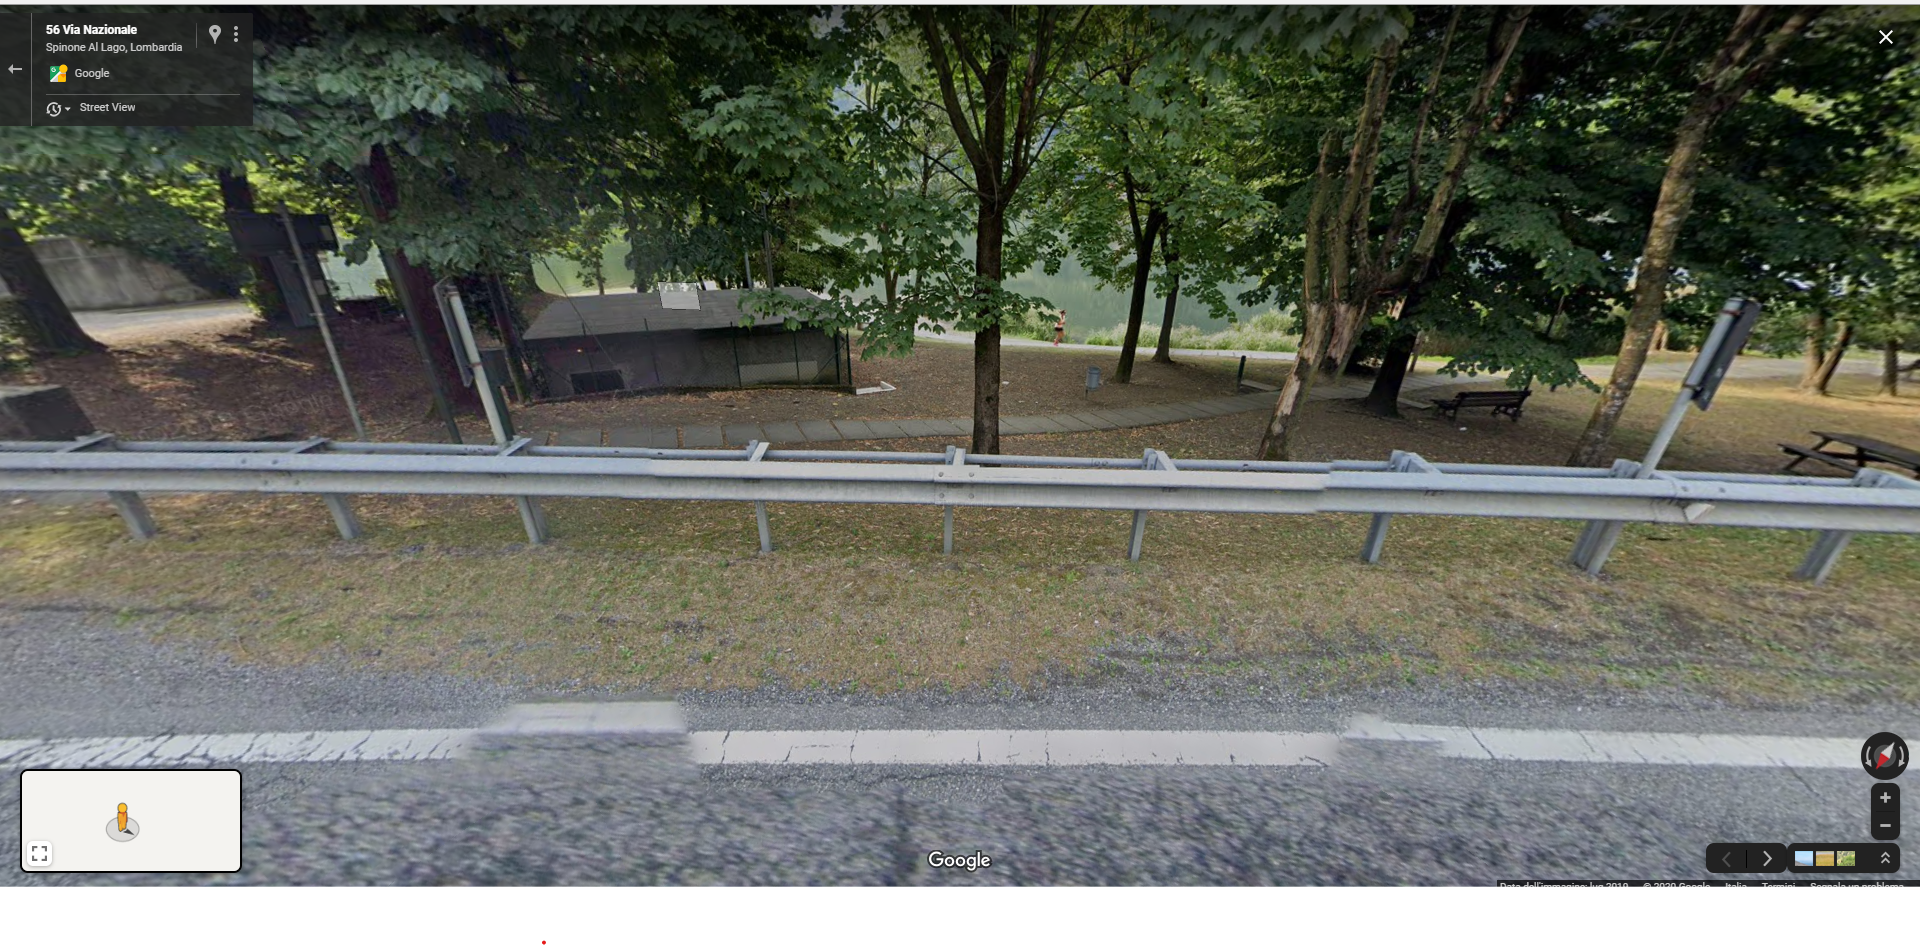
\includegraphics[width=0.8\textwidth]{image11}
	\caption{aaa}
	\label{fig:mesh1}
\end{figure}



Si tratta di  un edificio privato,dalle dimensioni di 4,30 x 5,40 metri, che in precedenza era adibito a rimessaggio per le barche.
Mi ha interessato la sua posizione perché dista pochi metri dal lago, è immersa in un ampio spazio verde, alberato  e situata di fronte alla pista pedonale.
Si tratta di un passaggio molto frequentato  che permette di percorrere tutto il lago. 
Nei periodi estivi e di bella stagione diventa un luogo di svago e relax per famiglie e gruppi di compagnie.
La zona circostante è pubblica ed è già allestita con tavoli e panchine.
Alle spalle passa un vialetto  che si congiunge alla strada principale, permettendo di raggiungere facilmente la struttura e offrendo dei parcheggi.

\subsection{Collocazione}

L’edificio per il rimessaggio si trova sul versante ovest del lago. Gode di un'ottima posizione ed esposizione alla luce solare.

\begin{figure}[H]
	\captionsetup[subfloat]{farskip=2pt,captionskip=8pt}
	\centering
	\subfloat[Mappa]{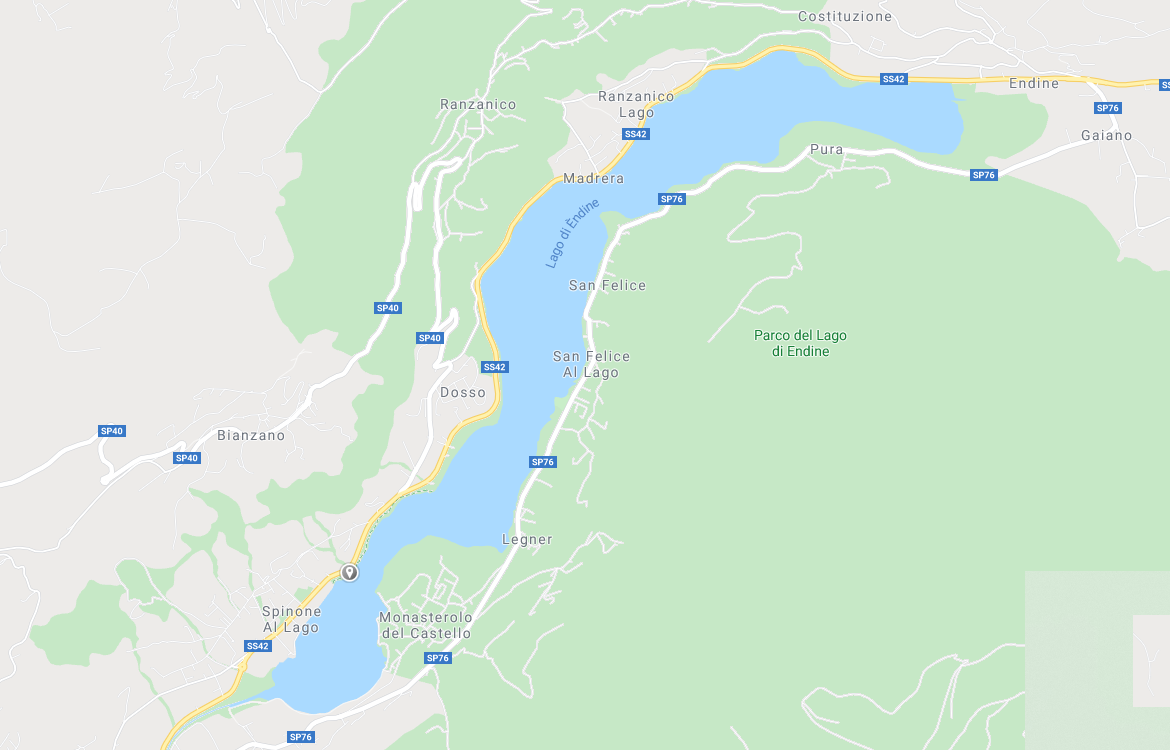
\includegraphics[width=6cm]{image12}}
	\hspace{1cm}
	\subfloat[Mappa aerea]{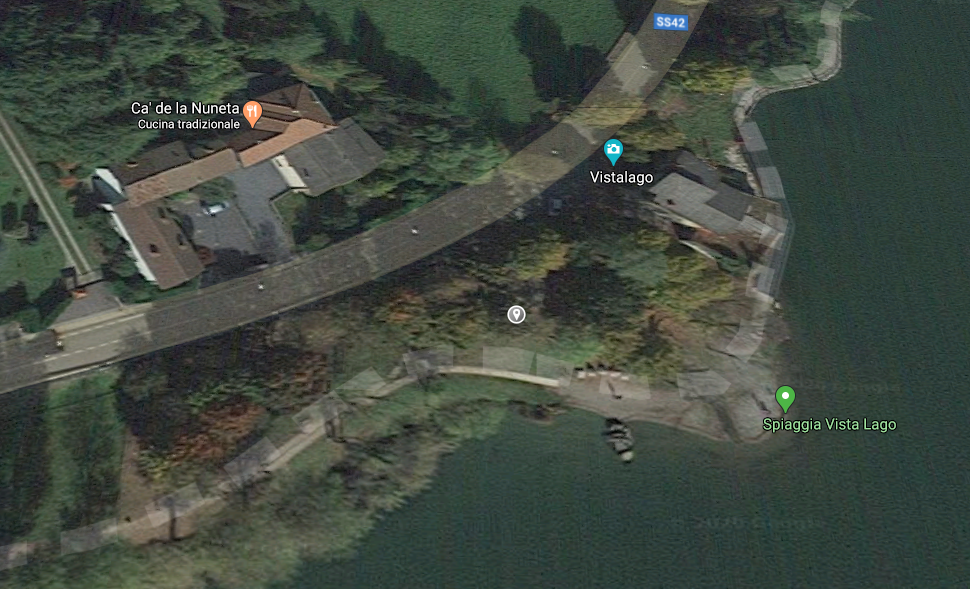
\includegraphics[width=6cm]{image24}}
	
	\caption{Mappe}
	\label{fig:imagesizes}
\end{figure}


\begin{figure}[H]
	\centering
	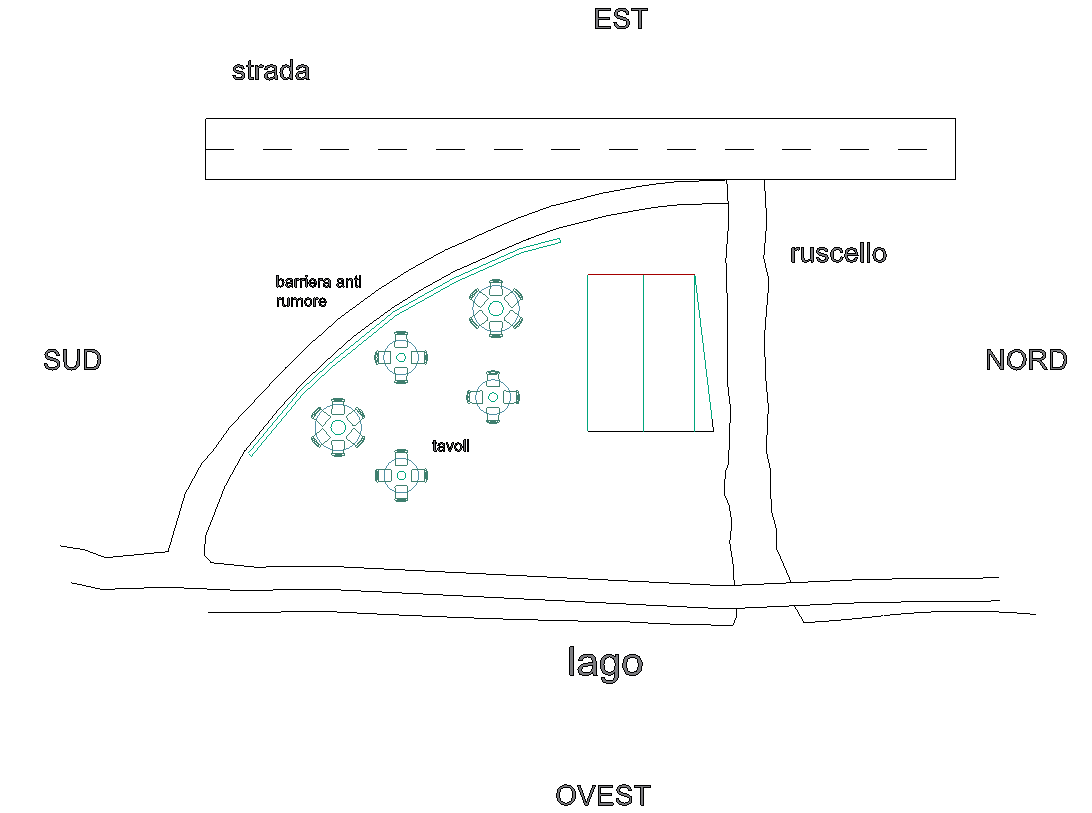
\includegraphics[width=0.8\textwidth]{image45}
	\caption{aaa}
	\label{fig:mesh1}
\end{figure}